\documentclass[a4paper, 14pt]{extreport}
\usepackage[T2A]{fontenc}
\usepackage[utf8]{inputenc}
\usepackage[english,russian]{babel}

\usepackage[left=2.5cm, right=1.5cm, top=2.5cm, bottom=2.5cm]{geometry}

\usepackage[tableposition=top,singlelinecheck=false]{caption}
\usepackage{subcaption}

\DeclareCaptionLabelFormat{gostfigure}{Рисунок #2}
\DeclareCaptionLabelFormat{gosttable}{Таблица #2}
\DeclareCaptionLabelSeparator{gost}{~---~}
\captionsetup{labelsep=gost}
\captionsetup*[figure]{labelformat=gostfigure}
\captionsetup*[table]{labelformat=gosttable}
\renewcommand{\thesubfigure}{\asbuk{subfigure}}

\usepackage{microtype}
\sloppy

\usepackage{setspace}
\onehalfspacing

\usepackage{indentfirst}
\setlength\parindent{5ex}

\usepackage{titlesec}
\titleformat{\chapter}{\LARGE\bfseries}{\thechapter}{20pt}{\Large}
\titleformat{\section}{\Large\bfseries}{\thesection}{20pt}{\large}

\addto{\captionsrussian}{\renewcommand*{\contentsname}{Содержание}}
\usepackage[square]{natbib}
\renewcommand{\bibsection}{\chapter*{Список литературы}}

\makeatletter
\def\@biblabel#1{#1. }
\makeatother

\usepackage{caption}

\usepackage{wrapfig}
\usepackage{float}
\usepackage{multirow}

\usepackage{graphicx}
\newcommand{\imgwc}[4]
{
  \begin{figure}[#1]
    \center{\includegraphics[width=#2]{inc/img/#3}}
    \caption{#4}
    \label{img:#3}
  \end{figure}
}
\newcommand{\imghc}[4]
{
  \begin{figure}[#1]
    \center{\includegraphics[height=#2]{inc/img/#3}}
    \caption{#4}
    \label{img:#3}
  \end{figure}
}
\newcommand{\imgsc}[4]
{
  \begin{figure}[#1]
    \center{\includegraphics[scale=#2]{inc/img/#3}}
    \caption{#4}
    \label{img:#3}
  \end{figure}
}

\usepackage{pgfplots}
\pgfplotsset{compat=newest}

\usepackage{minted}
\newminted{csh}{fontsize=\small, fontfamily=rm}

\usepackage{listings}
\usepackage{listingsutf8}
\lstset{
  language=csh,
  basicstyle=\footnotesize\ttfamily,
  keywordstyle=\color{blue},
  stringstyle=\color{red},
  commentstyle=\color{gray},
  numbers=left,
  numberstyle=\tiny,
  numbersep=5pt,
  frame=false,
  breaklines=true,
  breakatwhitespace=true,
  inputencoding=utf8
}

\newcommand{\code}[1]{\texttt{#1}}

\usepackage{amsmath}
\usepackage{amssymb}

\usepackage[unicode]{hyperref}
\hypersetup{hidelinks}

\makeatletter
\newcommand{\vhrulefill}[1]
{
  \leavevmode\leaders\hrule\@height#1\hfill \kern\z@
}
\makeatother



\begin{document}

\def\figurename{Рисунок}
 	
 	\begin{minipage}{0.2\textwidth}
 		
\includegraphics[scale=0.05]{bmstu.png}
 	\end{minipage}
 	\begin{minipage}{0.7\textwidth}
 		\small
 		\begin{center}
 			\textbf{Министерство науки и высшего образования Российской Федерации}
 			
 			\textbf{Федеральное государственное бюджетное образовательное учреждение высшего образования «Московский государственный технический университет имени Н.Э. Баумана}
 			
 			\textbf{(национальный исследовательский университет)»}
 			
 			\textbf{(МГТУ им. Н.Э. Баумана)}
 		\end{center}
 	\end{minipage}
 	
 	\vspace*{5mm}
 	
 	\normalsize
 	\begin{flushleft}
 		Факультет: <<Информатика и системы управления>>
 		
 		Кафедра: <<Программное обеспечение ЭВМ и информационные технологии>>
 	\end{flushleft}
 	
 	\vspace*{20mm}
 	
 	\LARGE
 	\begin{center}
 		\textbf{Расчетно-пояснительная записка}
 		
 		\textbf{к курсовой работе на тему:}
 		
 		\textbf{<<Создание веб-приложения, интернет-магазин животных>>}
 	\end{center}
 	
 	\vspace*{15mm}
 	
 	\large
 	\begin{flushleft}
 		\textbf{Студент:} Нечитайло Д.В. \\
 		\textbf{Группа:} ИУ7-66Б \\
 		%        \textbf{Оценка (баллы):} \\
 		\textbf{Научный руководитель:} Кивва К. А.
 	\end{flushleft}
 	
 	\vspace*{30mm}
 	
 	\large
 	\begin{center}
 		Москва, 2021 г.
 	\end{center}
 	
 	\thispagestyle{empty}
 	
 	\newpage

    \tableofcontents
    
\chapter*{Введение}
\addcontentsline{toc}{chapter}{Введение}
    \chapter{Аналитическая часть}

\section{Обзор и анализ существующих интернет-магазинов животных}

\hspace{0.6cm} В настоящее время большинство интернет-магазинов позволяют покупать продукцию для животных, узнавать информацию об услугах, имеют удобный и яркий интерфейс. Вот некоторые из них:

\begin{figure}[ht!]
  \centering
  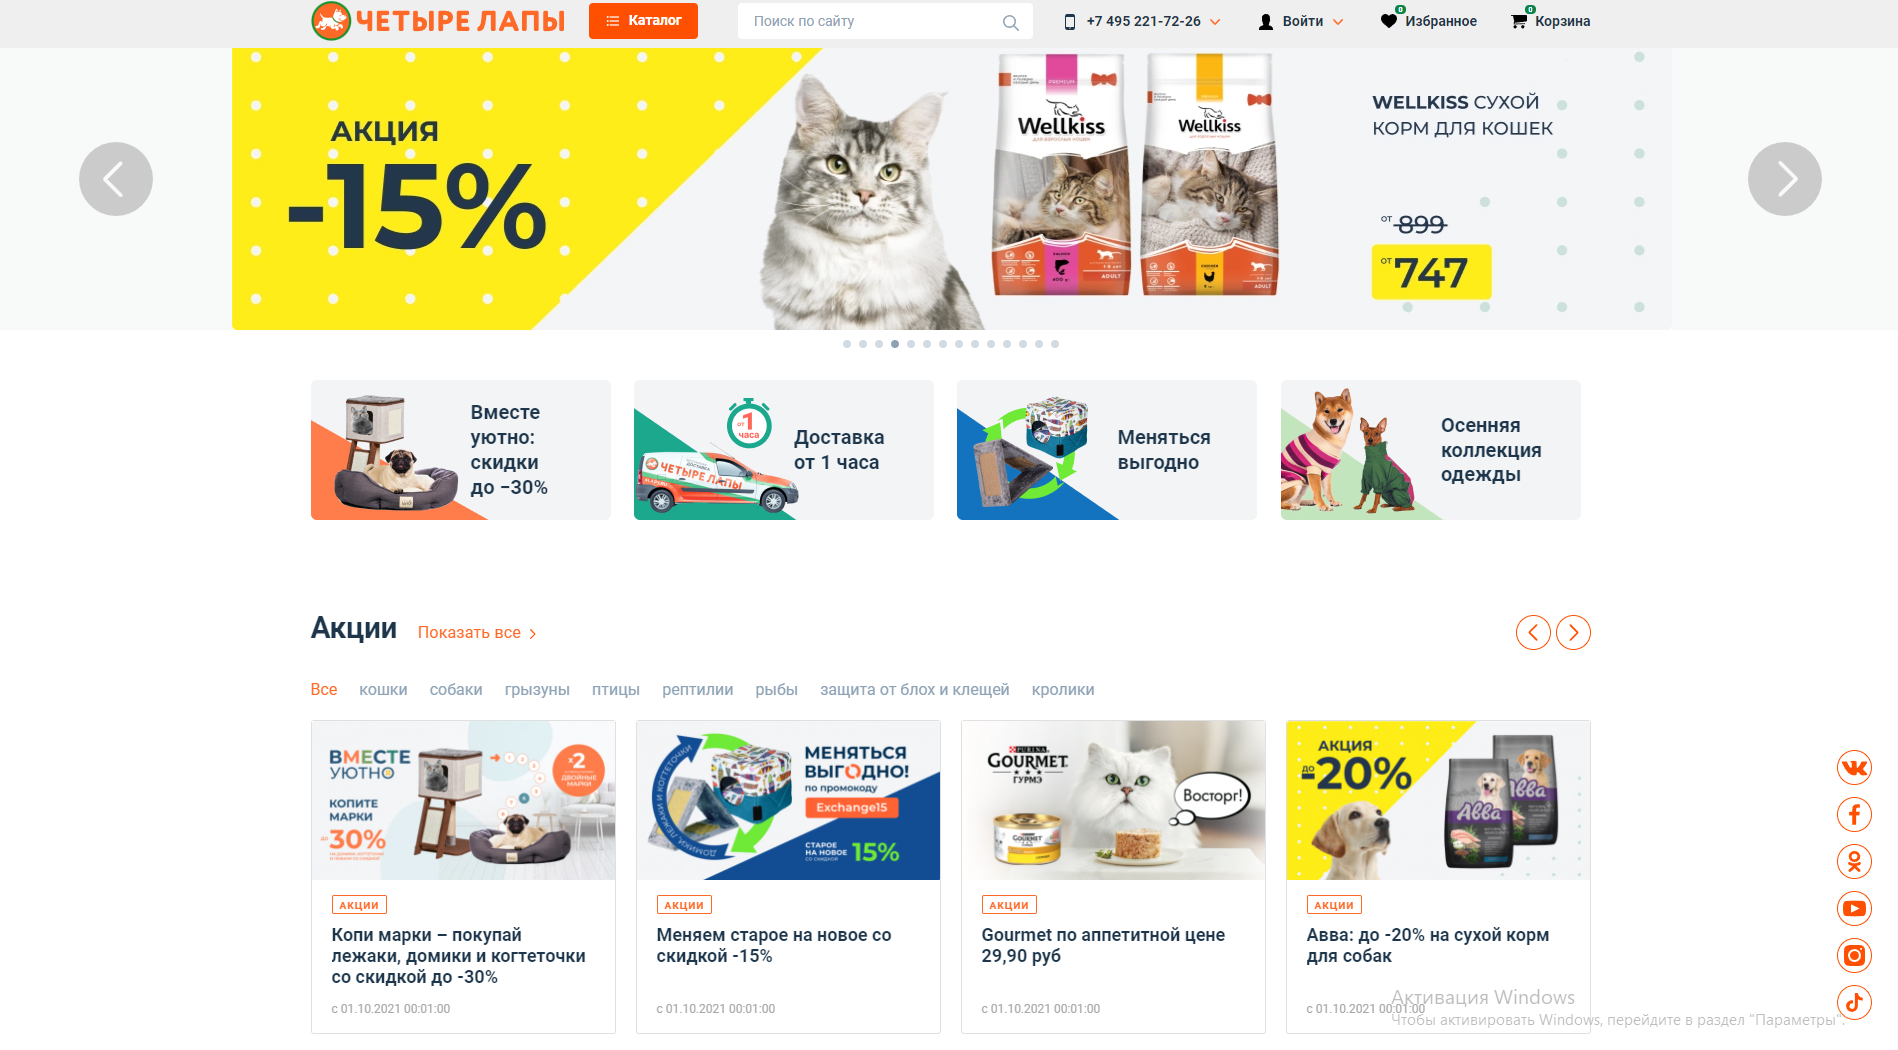
\includegraphics[scale=0.3]{chetirelapy.png}
  \caption{интернет-магазин Четыре Лапы}
  \label{fig:image1}
\end{figure}

\newpage

\begin{figure}[ht!]
  \centering
  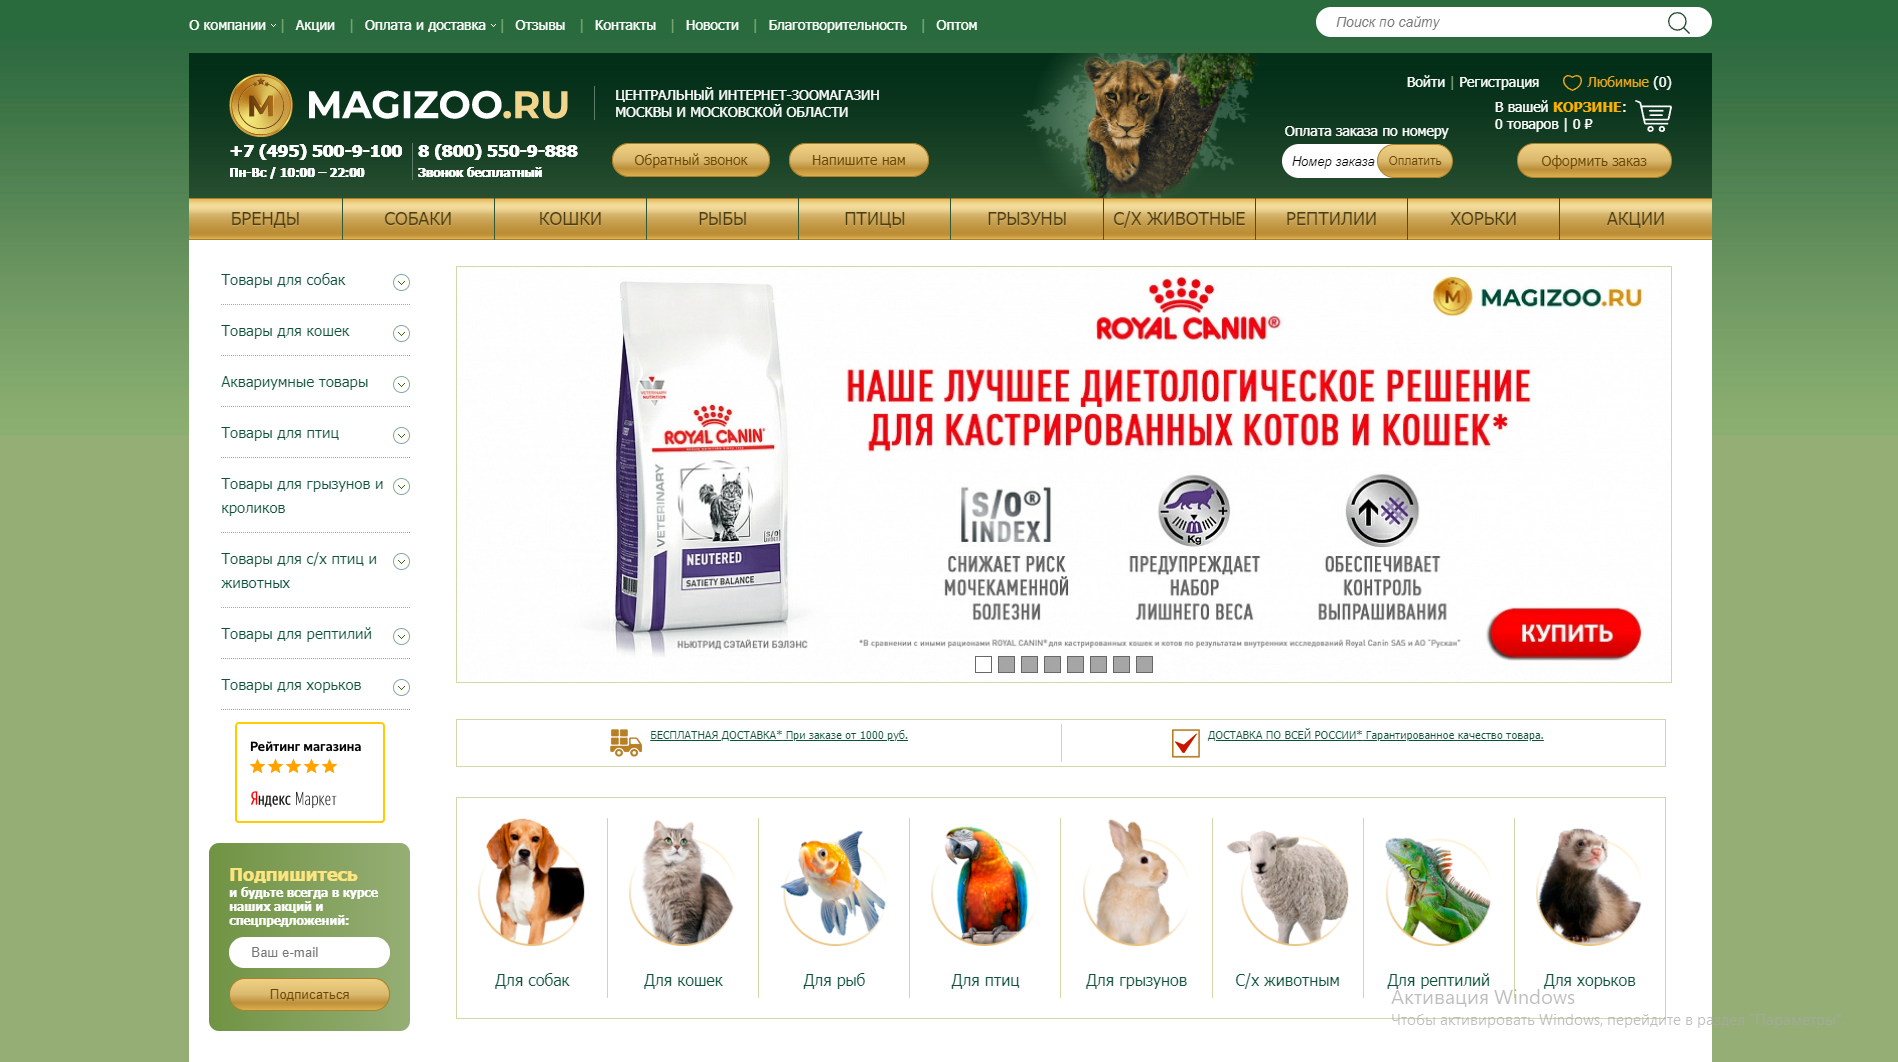
\includegraphics[scale=0.3]{magizoo.png}
  \caption{интернет-магазин Магизу}
  \label{fig:image2}
\end{figure}

\begin{figure}[ht!]
  \centering
  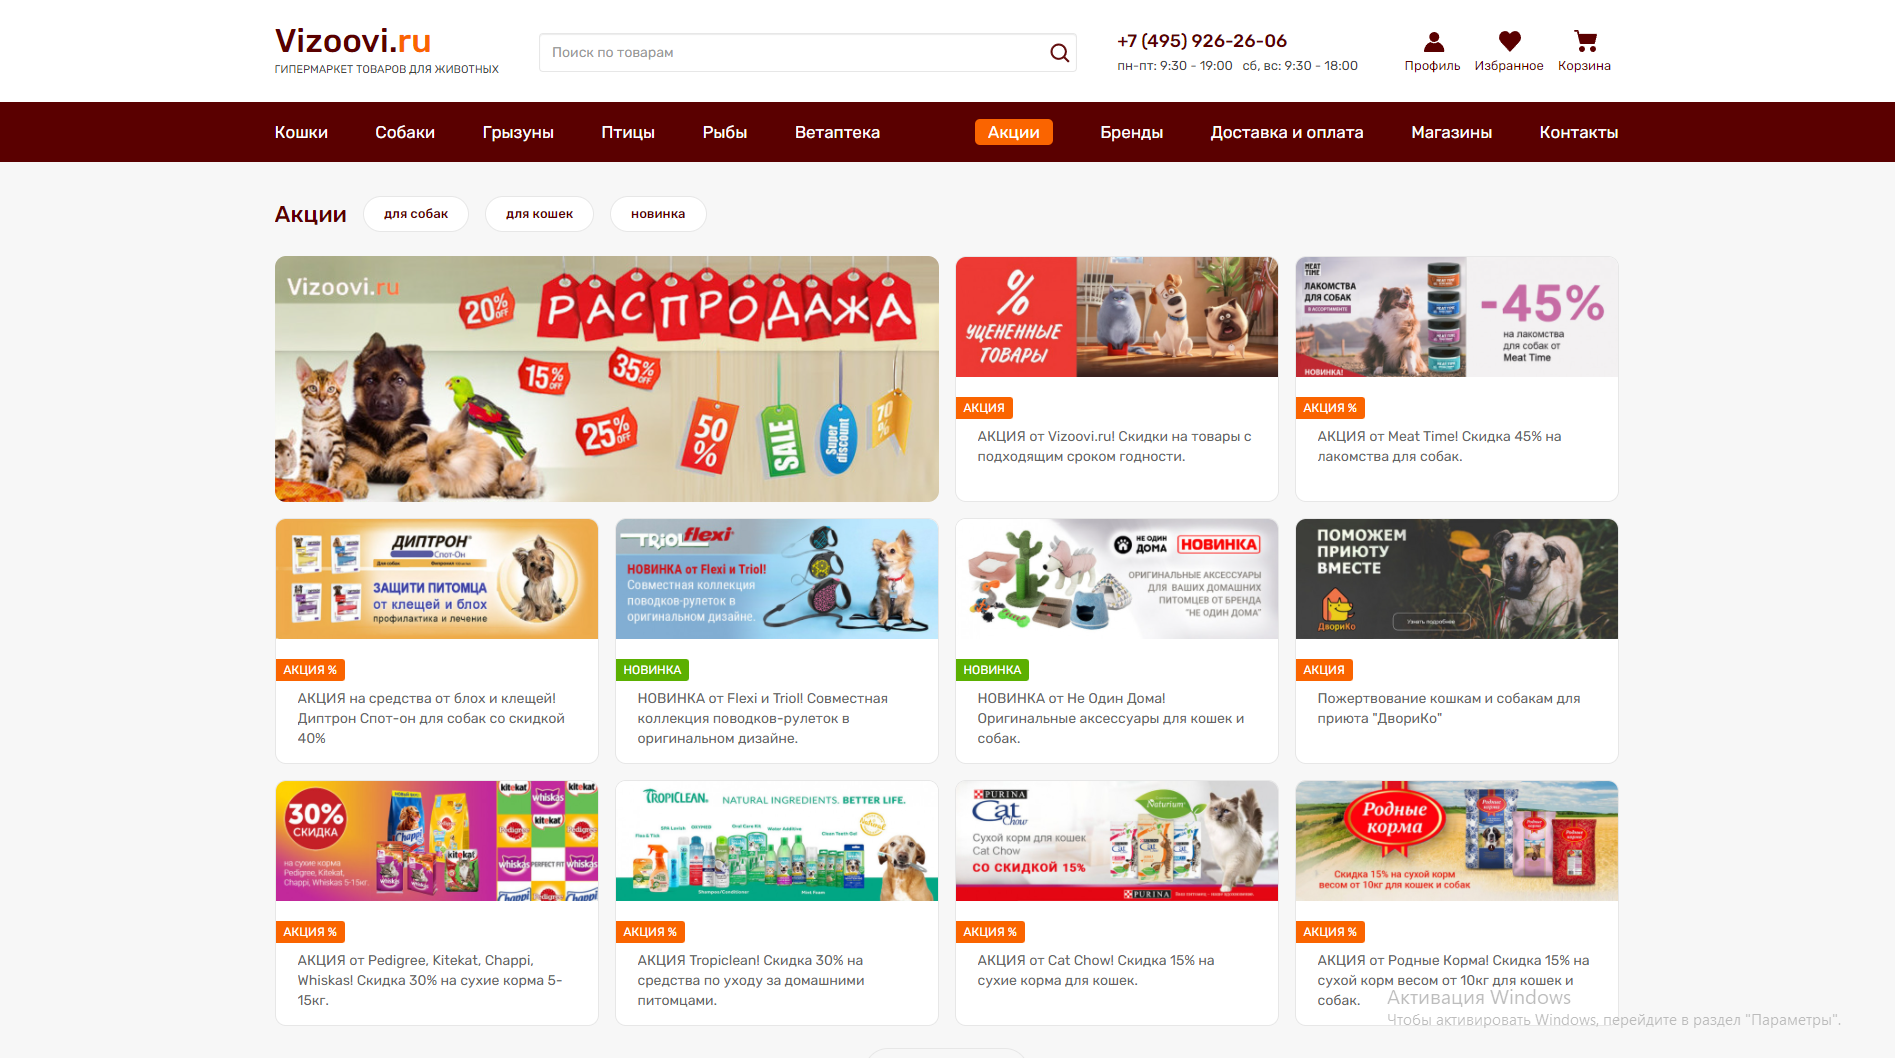
\includegraphics[scale=0.3]{vizoovi.png}
  \caption{интернет-магазин Визуви}
  \label{fig:image3}
\end{figure}

\newpage

\begin{figure}[ht!]
  \centering
  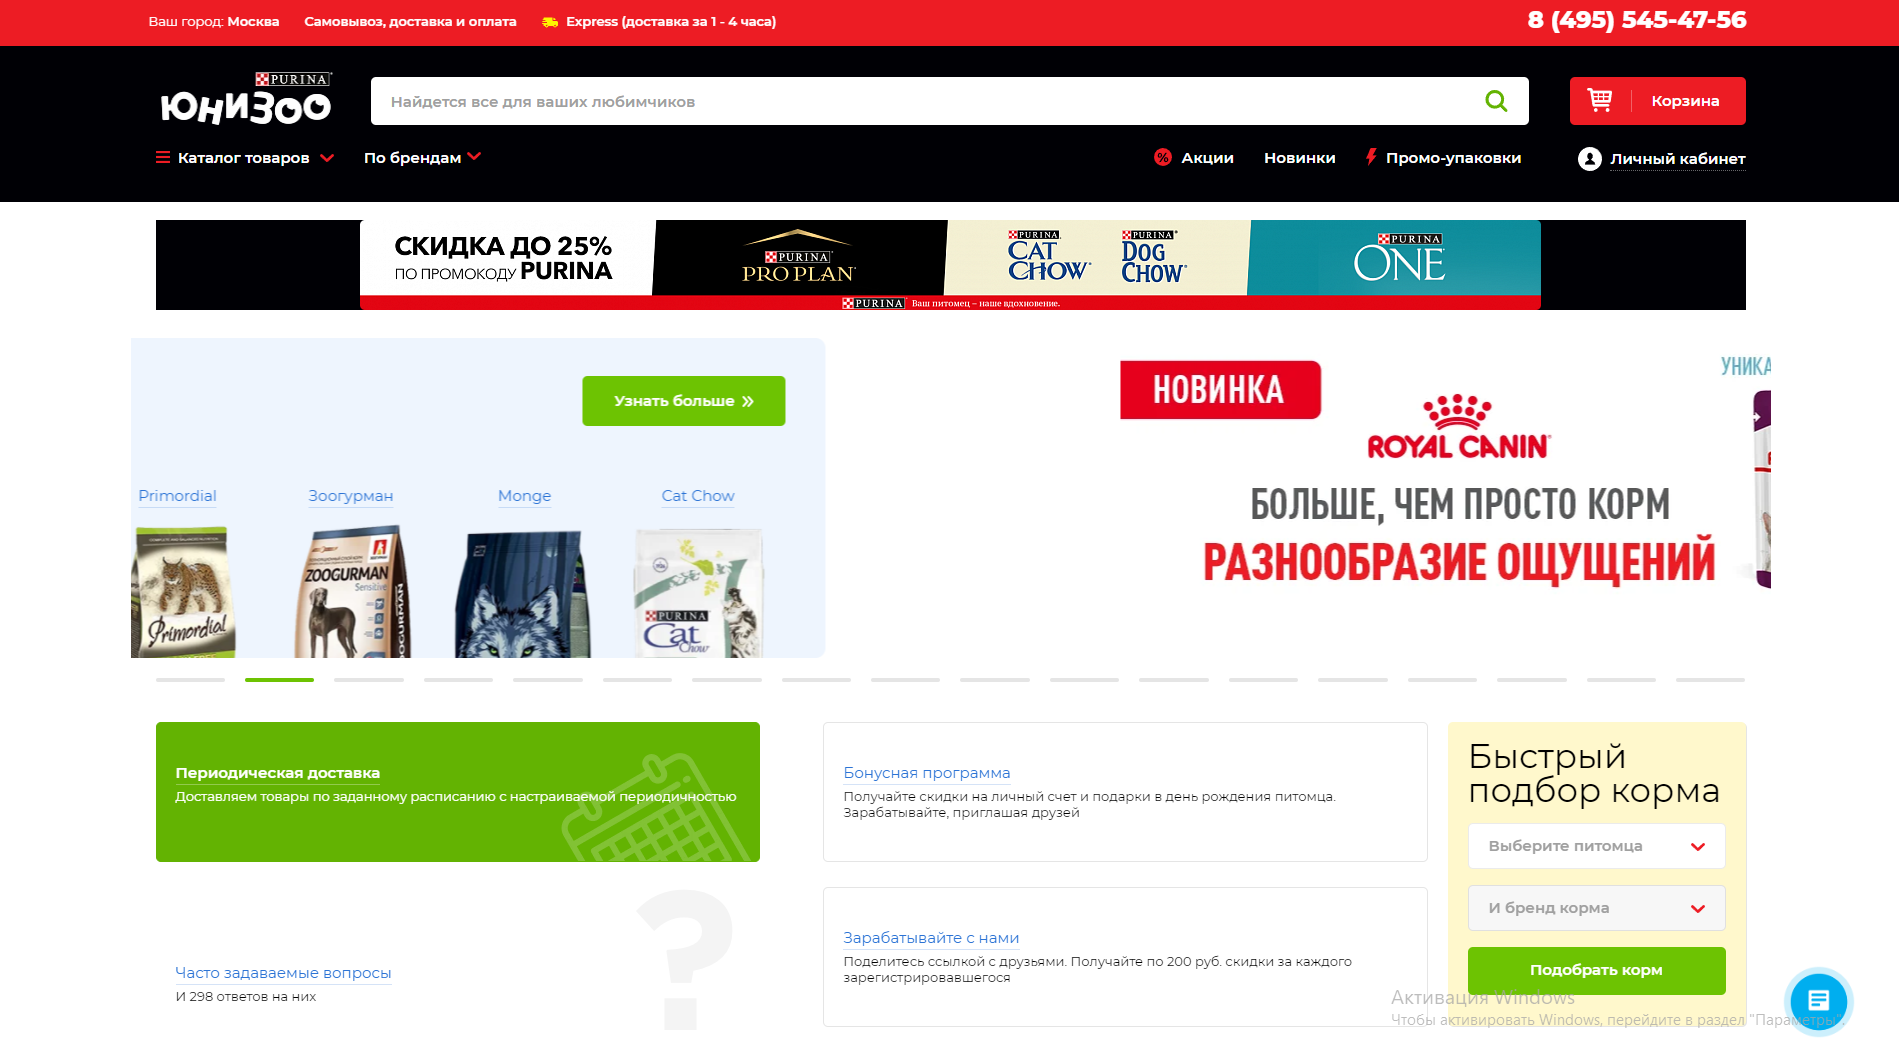
\includegraphics[scale=0.3]{unizoo.png}
  \caption{интернет-магазин Юнизу}
  \label{fig:image4}
\end{figure}

\hspace{0.6cm} Как можно заметить из рисунков \ref{fig:image1}, \ref{fig:image2}, \ref{fig:image3} и \ref{fig:image4}, в основном интерфейс магазинов отличается цветовой гаммой, использованной при создании визуальной составляющей, ассортиментом. Функционал предоставляемый на данных сайтах приблизительно одинаковый. Везде реализованы функции поиска товаров с возможностью фильтровать результат, регистрироваться и авторизоваться на сайте, для того чтобы иметь возможность сделать заказ. Однако в магазинах есть возможность покупать только товары для животных, а функционал предназначен только для покупателей.

\newpage

\hspace{0.6cm} На рисунке \ref{fig:image17} приведена use-case диаграмма, построенная основываясь на функционале приведенных ранее ресурсах. Данная схема составлена с целью отразить логику работы функций, предоставляемых ресурсами.

\begin{figure}[ht!]
  \centering
  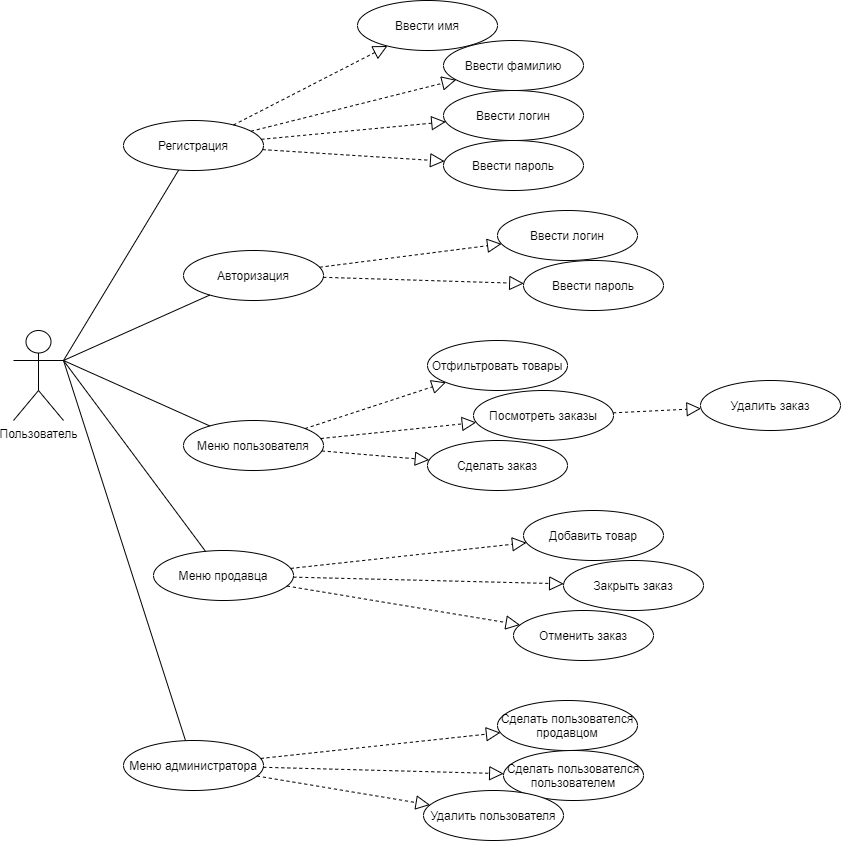
\includegraphics[scale=0.5]{Use-Case диаграмма.drawio.png}
  \caption{Use-Case диаграмма}
  \label{fig:image17}
\end{figure}

\section{Типы баз данных}

\hspace{0.6cm} База данных — это упорядоченный набор структурированной информации или данных, которые обычно хранятся в электронном виде в компьютерной системе. База данных обычно управляется системой управления базами данных (СУБД). Данные вместе с СУБД, а также приложения, которые с ними связаны, называются системой баз данных, или, для краткости, просто базой данных\cite{web:DBTypes}.

\hspace{0.6cm} Существует множество различных типов баз данных. Выбор наилучшей базы данных зависит от того, как и какие данные необходимо использовать.

\subsection{Реляционные базы данных}
Реляционные базы данных стали преобладать в 1980-х годах. Данные в реляционной базе организованы в виде таблиц, состоящих из столбцов и строк. Реляционная СУБД обеспечивает быстрый и эффективный доступ к структурированной информации. На рисунке \ref{fig:image7} приведен пример реляционной БД\cite{web:DBTypes}.

\begin{figure}[ht!]
  \centering
  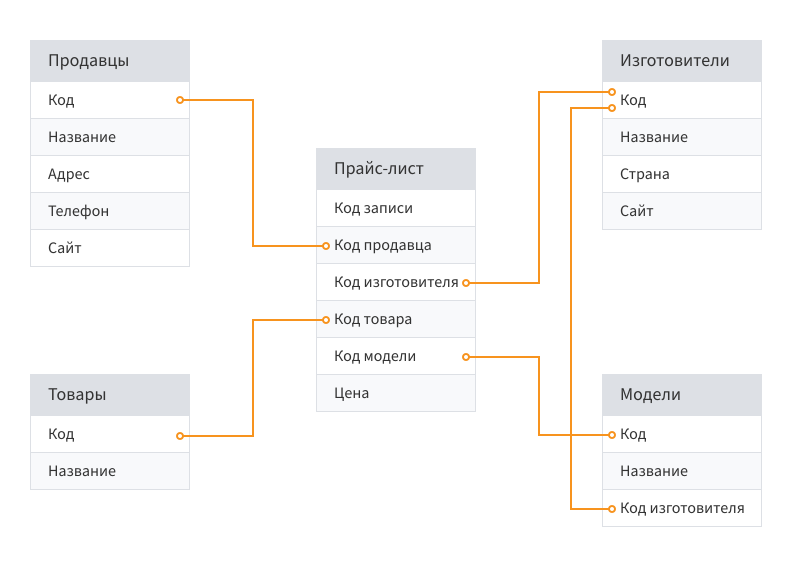
\includegraphics[scale=0.5]{relation-database.png}
  \caption{пример реляционной БД}
  \label{fig:image7}
\end{figure}

\newpage

\hspace{0.6cm} Преимущества:

\begin{itemize}
  \item Простота. В реляционной модели всего одна информационная конструкция, которая формализует табличное представление данных, привычное для пользователей;
  \item Теоретическое обоснование. Наличие теоретически обоснованных методов нормализации отношений позволяет получать БД с заданными характеристиками;
  \item Независимость данных. Когда необходимо изменить структуру реляционной БД, это, как правило, приводит к минимальным изменениям в прикладных программах;
\end{itemize}

\hspace{0.6cm} Недостатки:

\begin{itemize}
  \item Низкая скорость при выполнении операции соединения;
  \item Большой расход памяти для представления реляционной БД;
\end{itemize}

\subsection{Иерархические базы данных}
В Иерархическом типе БД появляются связи между объектами (записями). Каждая запись имеет одного «родителя». Это создаёт древовидную структуру, в которой записи классифицируются по их отношениям с цепочкой родительских записей\cite{web:IerarchiDB}. На рисунке \ref{fig:image12} приведен пример иерархичской бд.

 \begin{figure}[ht!]
  \centering
  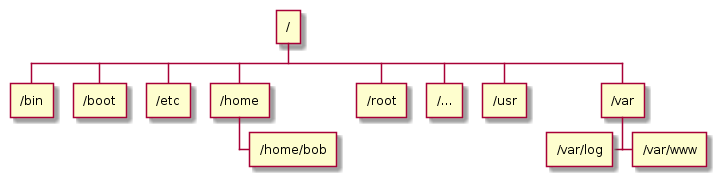
\includegraphics[scale=0.5]{IerarchiDB.png}
  \caption{пример иерархической базы данных}
  \label{fig:image12}
\end{figure}

\hspace{0.6cm} Преимущества:

\begin{itemize}
  \item простота понимания;
  \item простота оценки операционных характеристик.
\end{itemize}

\hspace{0.6cm} Недостатки:

\begin{itemize}
  \item могут быть избыточные данные;
  \item усложняются операции включения и удаления;
  \item удаление исходных объектов ведет к удалению порожденных объектов;
  \item процедурный характер манипулирования данными;
  \item доступ к любому порожденному узлу возможен только через корневой узел;
  \item сильная зависимость логической и физической БД;
  \item сильно ограниченный набор структур запроса.
\end{itemize}

\subsection{Сетевые базы данных}
Сетевые базы данных расширяют функциональность иерархических: записи могут иметь более одного родителя. А значит, можно моделировать сложные отношения. На рисунке \ref{fig:image11} приведен пример сетевой базы данных\cite{web:NetworkDB}.

 \begin{figure}[ht!]
  \centering
  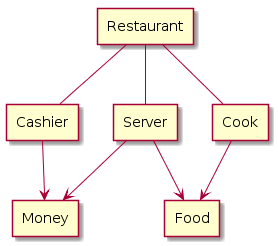
\includegraphics[scale=0.5]{networkDB.png}
  \caption{пример сетевой базы данных}
  \label{fig:image11}
\end{figure}

\hspace{0.6cm} Преимущества:

\begin{itemize}
  \item предоставляет большие возможности в смысле допустимости образования произвольных связей;
\end{itemize}

\hspace{0.6cm} Недостатки:

\begin{itemize}
  \item высокая сложность и жесткость схемы БД, сложность понимания и выполнения обработки информации;
\end{itemize}

\subsection{Графовые базы данных}
Графовая база данных хранит данные в контексте сущностей и связей между сущностями. На рисунке \ref{fig:image10} приведен пример графовой базы данных\cite{web:GraphDB}.

 \begin{figure}[ht!]
  \centering
  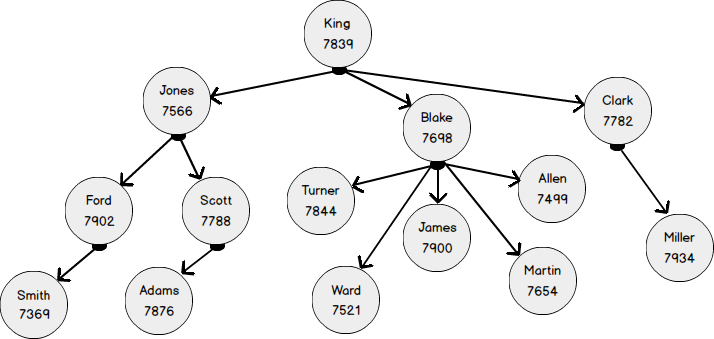
\includegraphics[scale=0.5]{GraphDB.png}
  \caption{пример графовой базы данных}
  \label{fig:image10}
\end{figure}

\hspace{0.6cm} Преимущества:

\begin{itemize}
  \item предоставляют чрезвычайно гибкую модель данных и способ развертывания, соответствующий современным способам развертывания программного обеспечения;
  \item производительность графовых баз данных остается неизменной с увеличением объема хранимых данных.
\end{itemize}

\hspace{0.6cm} Недостатки:

\begin{itemize}
  \item В базе данных графов каждая запись должна проверяться индивидуально во время запроса, чтобы определить структуру данных, в то время как в реляционной базе данных это известно заранее;
  \item база данных использует много места для хранения, потому что нужно хранить все отношения между записями.
\end{itemize}

\section{Выбор реляционных СУБД}

\subsection{SQLite}

\hspace{0.6cm} SQLite - Легко встраиваемая в приложения база данных. Так как это система базируется на файлах, то она предоставляет довольно широкий набор инструментов для работы с ней, по сравнению с сетевыми СУБД. При работе с этой СУБД обращения происходят напрямую к файлам (в эти файлах хранятся данные), вместо портов и сокетов в сетевых СУБД. Именно поэтому SQLite очень быстрая, а также мощная благодаря технологиям обслуживающих библиотек\cite{web:SQLite}.

\hspace{0.6cm} Преимущества:

\begin{itemize}
  \item файловая структура - вся база данных состоит из одного файла, поэтому её очень легко переносить на разные машины;
  \item используемые стандарты - хотя может показаться, что эта СУБД примитивная, но она использует SQL. Некоторые особенности опущены (RIGHT OUTER JOIN или FOR EACH STATEMENT), но основные все-таки поддерживаются;
  \item отличная при разработке и тестировании - в процессе разработки приложений часто появляется необходимость масштабирования. SQLite предлагает всё что необходимо для этих целей, так как состоит всего из одного файла и библиотеки написанной на языке C.
\end{itemize}

\hspace{0.6cm} Недостатки:

\begin{itemize}
  \item отсутствие системы пользователей - более крупные СУБД включают в свой состав системы управления правами доступа пользователей. Обычно применения этой функции не так критично, так как эта СУБД используется в небольших приложениях;
  \item отсутствие возможности увеличения производительности - опять, исходя из проектирования, довольно сложно выжать что-то более производительное из этой СУБД.
\end{itemize}

\subsection{PostgreSQL}

\hspace{0.6cm} PostgreSQL является самым профессиональным из всех трех рассмотренных нами СУБД. Она свободно распространяемая и максимально соответствует стандартам SQL. PostgreSQL или Postgres стараются полностью применять ANSI/ISO SQL стандарты своевременно с выходом новых версий\cite{web:PostgreSQL}.

\hspace{0.6cm} Преимущества:

\begin{itemize}
  \item открытое ПО соответствующее стандарту SQL - PostgreSQL - бесплатное ПО с открытым исходным кодом. Эта СУБД является очень мощной системой;
  \item большое сообщество - существует довольно большое сообщество в котором вы запросто найдёте ответы на свои вопросы;
  \item большое количество дополнений - несмотря на огромное количество встроенных функций, существует очень много дополнений, позволяющих разрабатывать данные для этой СУБД и управлять ими;
  \item расширения - существует возможность расширения функционала за счет сохранения своих процедур;
  \item объектность - PostrgreSQL это не только реляционная СУБД, но также и объектно-ориентированная с поддержкой наследования и много другого.
\end{itemize}

\hspace{0.6cm} Недостатки:

\begin{itemize}
  \item производительность - при простых операциях чтения PostgreSQL может значительно замедлить сервер и быть медленнее своих конкурентов, таких как MySQL;
  \item популярность - по своей природе, популярностью эта СУБД похвастаться не может, хотя и присутствует довольно большое сообщество;
  \item хостинг - в силу выше перечисленных факторов иногда довольно сложно найти хостинг с поддержкой этой СУБД.
\end{itemize}

\subsection{MySQL}

\hspace{0.6cm} MySQL - это самая распространенная полноценная серверная СУБД. MySQL очень функциональная, свободно распространяемая СУБД, которая успешно работает с различными сайтами и веб приложениями. Обучиться использованию этой СУБД довольно просто, так как на просторах интернета вы легко найдете большее количество информации\cite{web:SQLite}.

\hspace{0.6cm} Преимущества:

\begin{itemize}
  \item простота в работе - установить MySQL довольно просто. Дополнительные приложения, например GUI, позволяет довольно легко работать с БД;
  \item богатый функционал - MySQL поддерживает большинство функционала SQL;
  \item безопасность - большое количество функций обеспечивающих безопасность, которые поддерживается по умолчанию;
  \item масштабируемость - MySQL легко работает с большими объемами данных и легко масштабируется;
  \item скорость - упрощение некоторых стандартов позволяет MySQL значительно увеличить производительность.
\end{itemize}

\hspace{0.6cm} Недостатки:

\begin{itemize}
  \item известные ограничения - по задумке в MySQL заложены некоторые ограничения функционала, которые иногда необходимы в особо требовательных приложениях;
  \item проблемы с надежностью - из-за некоторых способов обработки данных MySQL (связи, транзакции, аудиты) иногда уступает другим СУБД по надежности;
  \item медленная разработка - Хотя MySQL технически открытое ПО, существуют жалобы на процесс разработки. Стоит заметить, что существуют другие довольно успешные СУБД созданные на базе MySQL, например MariaDB.
\end{itemize}

\subsection{MariaDB}

\hspace{0.6cm} MariaDB – это по-настоящему открытый дистрибутив MySQL (выпущен под GNU GPLv2). Он был создан после приобретения Oracle MySQL, когда некоторые из основных разработчиков MySQL были обеспокоены тем, что Oracle подорвет его философию открытого исходного кода.

\hspace{0.6cm} MariaDB был разработан, чтобы быть максимально совместимым с MySQL при замене нескольких ключевых компонентов. Он использует механизм хранения Aria, который функционирует как транзакционный, так и нетранзакционный механизм. Некоторые даже предполагали, что Aria станет стандартным движком для MySQL в будущих выпусках, прежде чем MariaDB станет независимым проектом\cite{web:MariaDB}.

\hspace{0.6cm} Преимущества:

\begin{itemize}
  \item многие пользователи выбирают MariaDB вместо MySQL из-за частых обновлений систем безопасности MariaDB. Хотя это не обязательно означает, что MariaDB более безопасна, это означает, что сообщество разработчиков серьезно относится к безопасности;
  \item другие говорят, что основные преимущества MariaDB в том, что она почти наверняка останется с открытым исходным кодом и будет полностью совместима с MySQL. Это означает, что миграция из одной системы в другую происходит очень быстро;
  \item благодаря этой совместимости MariaDB также хорошо работает со многими другими языками, которые обычно используются в MySQL. Это означает, что на изучение и отладку кода тратится меньше времени;
  \item можно установить и запустить WordPress с MariaDB вместо MySQL для лучшей производительности и более богатого набора функций. WordPress является самой популярной CMS от markethare, которая обеспечивает почти половину контента в интернете, и имеет активное сообщество разработчиков с открытым исходным кодом. Сторонние темы и плагины работают так, как задумано, когда WordPress установлен с MariaDB.
\end{itemize}

\hspace{0.6cm} Недостатки:

\begin{itemize}
  \item MariaDB несколько подвержен «вздутию живота». Его центральный файл журнала IDX, в частности, имеет тенденцию становиться очень большим после длительного использования, что в конечном итоге снижает производительность;
  \item кэширование – это еще одна область, в которой MariaDB могла бы усовершенствоваться. Этот процесс не такой быстрый, каким мог бы быть, что немного расстраивает;
  \item несмотря на все первоначальные обещания, MariaDB больше не полностью совместима с MySQL. Если вы переходите с MySQL, вам нужно будет выполнить перекодировку.
\end{itemize}

\newpage

\section{Вывод}

\hspace{0.6cm} Проанализировав существующие ресурсы для покупки питомцев, было решено создать веб-приложение, в котором будет реализован функционал представленный в ресурсах, а также функционал для продавцов, с возможностью обрабатывать заказы и администратора, для осуществления контроля за продавцами и покупателями. На основании анализа предметной области была построена ER-диаграмма, продемонстрированная на рисунке \ref{fig:image16}.

 \begin{figure}[ht!]
  \centering
  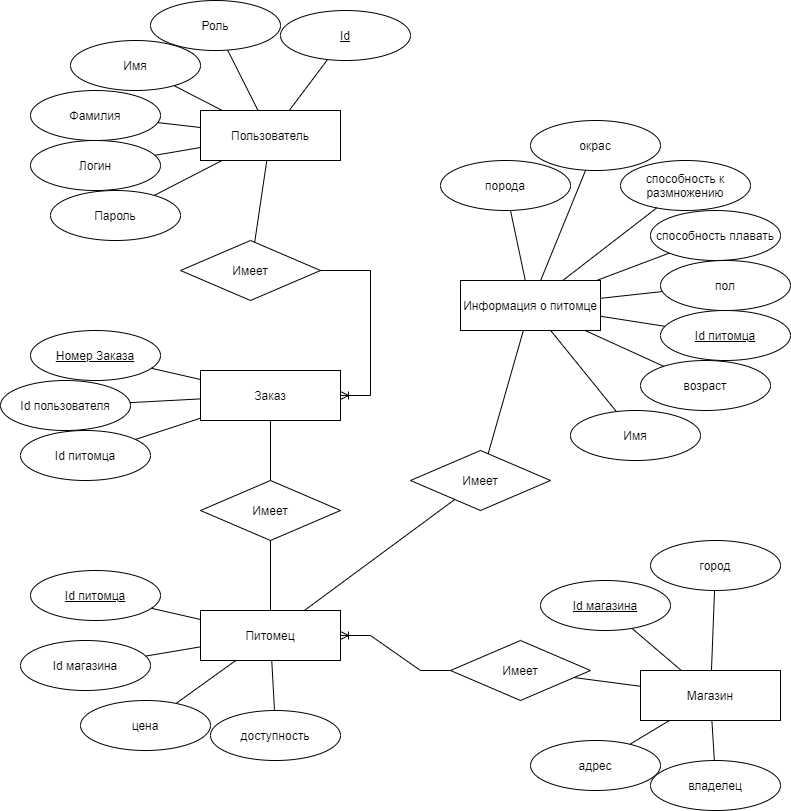
\includegraphics[scale=0.5]{ER-модель.drawio.png}
  \caption{ER-диаграмма}
  \label{fig:image16}
\end{figure}

\newpage

\hspace{0.6cm} Проанализировав все варианты типов БД, было решено выбрать реляционную базу данных и работать с СУБД MySQL. Достоинства данной модели:

\begin{itemize}
  \item простота в работе - установить MySQL довольно просто. Дополнительные приложения, например GUI, позволяет довольно легко работать с БД;
  \item богатый функционал - MySQL поддерживает большинство функционала SQL;
  \item безопасность - большое количество функций обеспечивающих безопасность, которые поддерживается по умолчанию;
  \item масштабируемость - MySQL легко работает с большими объемами данных и легко масштабируется;
  \item скорость - упрощение некоторых стандартов позволяет MySQL значительно увеличить производительность.
\end{itemize}




    \chapter{Конструкторская часть}

\section{Структура БД}

\subsection{Описание таблиц БД}

\hspace{0cm} База данных состоит из 5 таблиц: Users, Orders, Pets, Pet\_info, Shops.

\hspace{0cm} Users – таблица, в которой хранится логин и пароль пользователя, его имя и фамилия, а также роль. Полномочия пользователя определяется ролью. Customer – роль покупателя, который может создавать или отменять заказы, просматривать ассортимент магазина. Vendor – роль продавца работающего с заказами покупателей, способный их закрывать и отменять, добавлять новые товары. Каждый User может создать много Order(заказов).

\hspace{0cm} Orders - таблица, в которой хранится уникальный номер заказа, индентификационный номер пользователя создавшего заказ и индентификационный номер животного, которое пользователь закал. Один заказ может быть оформлен только на одно животное. Пользователь может создавать сколько угодно заказов.

\hspace{0cm} Pets - таблица, в которой хранится цена животного, его индентификационный номер, индентификационный номер магазина, в котором данный питомец в наличии, а также спецальное поле, которое определяет доступно ли животное для заказа или нет.

\hspace{0cm} Pet\_info - таблица, в которой хранится вся дополнительная информация о животном, такая как окрас, порода, возраст, возможность плавать или размножаться.

\hspace{0cm} Shops - таблица, в которой хранится информация о магазинах животных, их адресах, городах и владельцах.

\subsection{Описание полей БД}

Users

\begin{itemize}
  \item User\_id int – уникальный идентификатор пользователя, целочисленный тип, является первичным ключем;
  \item Login varchar(100) – логин пользователя, строковый тип;
  \item Password varchar(100) – пароль пользователя, строковый тип;
  \item Name varchar(100) – имя пользователя, строковый тип;
  \item Surname varchar(100) – фамилия пользователя, строковый тип;
  \item Role enum(‘admin’,’customer’,’vendor’) – роль пользователя, группа строковых значений.
\end{itemize}

Orders

\begin{itemize}
  \item Order\_number int – уникальный номер заказа,  целочисленный тип, является первичным ключем;
  \item User\_id int – уникальный идентификатор пользователя, целочисленный тип;
  \item Pet\_id int – уникальный идентификатор питомца, целочисленный тип.
\end{itemize}

Pets

\begin{itemize}
  \item Pet\_id int – уникальный идентификатор питомца, целочисленный тип, является первичным ключем;
  \item Shop\_id int – уникальный идентификатор магазина, целочисленный тип;
  \item Price int – цена животного, целочисленный тип;
  \item Available enum(‘yes’,’no’) – доступность питомца для заказа, группа строковых значений.
\end{itemize}

Pet\_info

\begin{itemize}
  \item Pet\_id int – уникальный идентификатор питомца, целочисленный тип, является первичным ключем;
  \item Pet\_type enum(‘Cat’,’Dog’,’Raccoon’,’Hedgehog’,’Fox’) – , группа строковых значений;
  \item Name varchar(100) – кличка животного, строковый тип;
  \item Age int – возраст животного, целочисленный тип;
  \item Color varchar(100) – цвет животного, строковый тип;
  \item Can\_swim bit – умение плавать, тип принимающий значения 1 или 0;
  \item Reproduce\_ability bit – способность животного к размножению, тип принимающий значения 1 или 0;
  \item Gender enum(‘Male’,’Female’) – пол животного, группа строковых значений;
  \item Pet\_breed varchar(100) – порода животного, строковый тип.
\end{itemize}

Shops

\begin{itemize}
  \item Shop\_id int – уникальный идентификатор магазина, целочисленный тип, является первичным ключем;
  \item Address varchar(100) – адрес магазина, строковый тип;
  \item City varchar(100) – город, в котором находится магазин, строковый тип;
  \item Owner varchar(100) – имя и фамилия владельца магазина, строковый тип.
\end{itemize}

\newpage

\subsection{Классы на основе таблиц БД}

\hspace{0cm} Чтобы работать с результатом запросов в БД, было решено создать под каждую таблицу.

\hspace{0cm} Users – объект, в котором хранится информация о пользователе, имя, фамилия, логин и пароль, для каждого пользователя существует один такой объект. Так же в нем находится роль пользователя (продавец, покупатель, администратор).

\hspace{0cm} Orders - объект, в котором хранится информация о заказе, пользователе сделавшем его и питомце, который был заказан. В нем находится идентификационный номер пользователя и питомца, а так же уникальный номер заказа.

\hspace{0cm} Pets - объект, в котором хранится информация о цене животного, его доступности в магазине, а так же идентификационный номер магазина, где его можно купить и самого животного.

\hspace{0cm} Pet\_info - объект, в котором хранится информация о питомце, такая как возраст, окрас, порода, умение плавать или иметь потомство, пол.

\hspace{0cm} Shops - объект, в котором хранится информация о магазинах, их владельцах, адресах и городах, в которых они располагаются.


\subsection{Схема БД}

\hspace{0cm} На рисунке \ref{fig:image6}, приведенном ниже, схема БД с учетом всех полей и таблиц, описанных в подпунктах выше.

\begin{figure}[ht!]
  \centering
  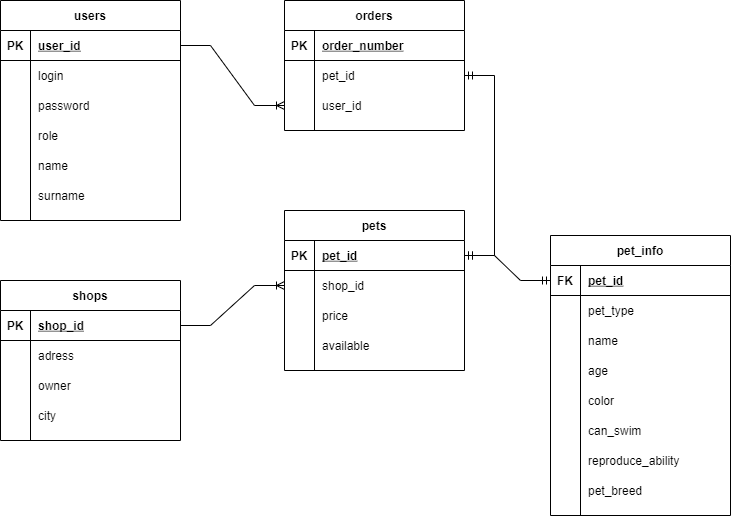
\includegraphics[scale=0.5]{img/Схема БД.drawio.png}
  \caption{Схема БД}
  \label{fig:image6}
\end{figure}

\newpage

\section{Архитектура программного обеспечения}

\hspace{0cm} В соответствии с техническим заданием будущее приложение должно иметь систему MVC(model, view, controller): веб-приложение(представление/view), базу данных(модель/model) и логику на серверную части(контроллер/controller). Основная цель применения этой концепции состоит в отделении бизнес-логики(модели) от её визуализации. За счёт такого разделения повышается возможность повторного использования кода.

\hspace{0cm} Основываясь на рисунке \ref{fig:image17} и модели MVC будет создаваться программа. Для каждого пункта доступного пользователю, а точнее: регистрация, авторизация, меню пользователя, меню продавца и меню администратора будет необходимо создать отдельный как контроллер, так и представление.

\hspace{0cm} Контроллер представляет из себя часть кода, которая отвечает за свое представление, передачу, получение и обработку данных с него, а так же взаимодействие с БД в случае необходимости добавления, удаления или изменения данных в ней.

\hspace{0cm} Функции работы с моделью (базой данных) храняться и реализовываются отдельно от контроллеров, однако предоставляют возможность к ним обращаться любым контроллерам. Каждая таблица при необходимости работы с ней имеет свое отдельное представление на уровне программы в виде класса или структуры данных. Это делается для более эфективной работы с данными.

\hspace{0cm} Представление связано со своим контроллером. Само представление является визуальной состовляеющей веб-приложения. Оно предоставялет возможность вводить пользователю данные, пользоваться функционалом посредством виджетов(кнопок), а также просматривать необходимую информацию.

\hspace{0cm} Обмен данными между представлением и контроллером происходит через HTTP запросы put для передачи, например логина и пароля при авторизации и get для вызова функций на стороне котроллера.

\begin{figure}[ht!]
  \centering
  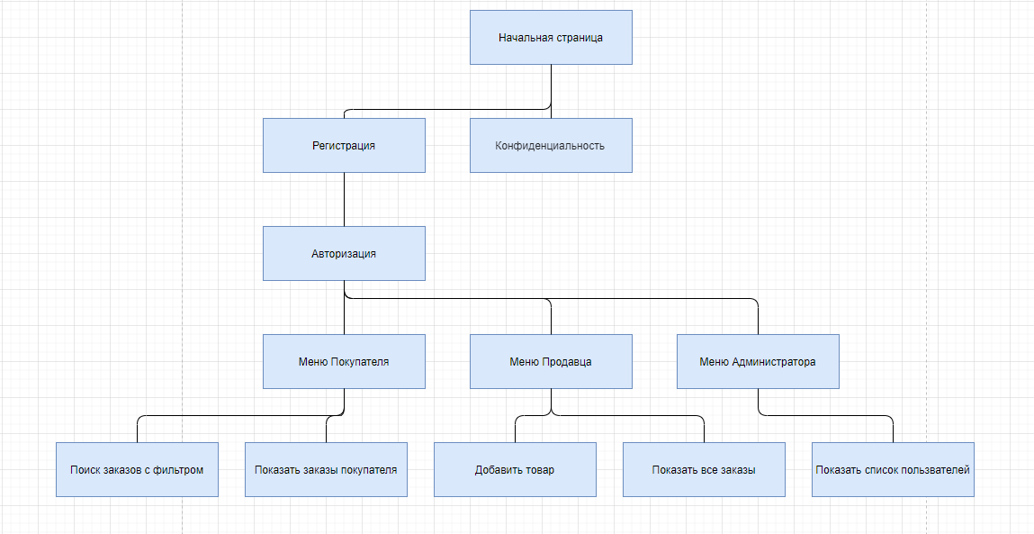
\includegraphics[scale=0.5]{img/Схема Работы ПО.png}
  \caption{С}
  \label{fig:image21}
\end{figure}

\hspace{0cm} На рисунке \ref{fig:image21} изображена спроектированная схема работы ПО, в которой можно увидеть взаимосвязь разных окон.

\hspace{0cm} Начальная страница, авторизация, регистрация, меню покупателя, продавца и администратора будут иметь каждый свой отдельный контроллер и представление. Оставшиеся на рисунке функции будут реализовываться вместе с тем меню, с которым связаны, то есть их внешний вид будет частью представления определенного меню, а функции обработки будут находиться в соответсвующем контроллер. Например функция "добавить товар" будет являеться частью меню продавца.

\section{Выводы}

\hspace{0cm} В данном разделе были представлены схемы и диаграммы, представляющие структуру БД, а также описывающая логику её работы. Так же были показаны диаграммы работы системы ПО.


    \chapter{Технологическая часть}

\section{Выбор среды и языка разработки}

\hspace{0cm} В качестве языка был выбран c\#, а вместе с ним и среда для разработки Visual Studio 2019. Так выбор был сделан в связи с:

\begin{itemize}
  \item Удобством удобством разработки, большим количеством вспомогательных функций (например, проверка синтаксиса);
  \item Наличием наличием диспетчера пакетов Nuget, позволяющего быстро добавлять необходимые расширения, без трат времени на долгий поиск и внедрение;
  \item Обозревателем обозревателем решений, позволяющим быстро переключаться между файлами в проекте.
\end{itemize}


\section{Используемые инструменты и технологии веб-приложения}

\hspace{0cm} В качестве фреймворка был выбран ASP.NET MVC. Причиной такого выбора стали:

\begin{itemize}
  \item Для данной задачи необходима реализации системы MVC, а данный фреймворк служит именно для этой цели;
  \item Наличие возможности реализовать Front-end вместе с Back-end используя HTML+CSS+C\#.
\end{itemize}

\hspace{0cm} Чтобы работать с базой данных через веб-приложение на C\# существует несколько вариантов:

\begin{itemize}
  \item Entity Framework — это решение для работы с базами данных, которое используется в программировании на языках семейства.NET. Оно позволяет взаимодействовать с СУБД с помощью сущностей (entity), а не таблиц. Также код с использованием EF пишется гораздо быстрее;
  \item MySQLConnector – динамическая библиотека предоставляющая возможность подключения и работы с MySql;
  \item MySQLData – динамическая библиотека предоставляющая возможность подключения и работы с MySql.
\end{itemize}

\hspace{0cm} Поскольку в качестве фреймворка был уже выбран ASP.net, удобнее выбрать динамическую библиотеку, поэтому была использована MySQLData. Для хостинга локального MySql сервера используется приложение MAMP.

\section{Реализация}

\hspace{0cm} При работе с базой устанавливается соединение с помощью строки подключения и функции динамической библиотеки MySQlData. Получение данных происходит после отправки запроса в СУБД. Запрос пишется на языке SQL. Работа с данными на серверной части осуществляется при помощи классов моделей, которые структурно совпадают с таблицами или с необходимым для нас выводом. Приложение при запуске начинает прослушивать порт 5001, по ip 127.0.0.1.

\section{Модель хранения}

На листингах \ref{list:user} и \ref{list:pet_info} представлены реализации классов user и pet\_info в программе.

\begin{lstlisting}[caption=класс User, label=list:user]
public int id { get; set; }
public string login { get; set; }
public string password { get; set; }
public string name { get; set; }
public string surname { get; set; }
public string role { get; set; }
\end{lstlisting}

\begin{lstlisting}[caption=класс pet\_info, label=list:pet_info]
public int pet_id { get; set; }
public string pet_type { get; set; }
public string name { get; set; } 
public int age { get; set; } 
public string color { get; set; } 
public int can_swim { get; set; } 
public int reproduce_ability { get; set; } 
public string gender { get; set; } 
public string pet_breed { get; set; } 
\end{lstlisting}

На листингах ниже представлены реализации запросов в базу данных.
Листинг \ref{list:GetUsers} – получение всех пользователей, листинг \ref{list:GetPetById} получение питомца по id.

\begin{lstlisting}[caption=функция получения всех пользователей, label=list:GetUsers]
public List<User> GetUsers()
{
    string sql = "SELECT * FROM `users`";

    cmd = new MySqlCommand();
    cmd.Connection = conn;
    cmd.CommandText = sql;

    var users = new List<User>();

    using (DbDataReader reader = cmd.ExecuteReader())
    {
        if (reader.HasRows)
        {
            while (reader.Read())
            {
                int userId = Convert.ToInt32(reader.GetValue(reader.GetOrdinal("user_id")));
                string login = reader.GetString(reader.GetOrdinal("login"));
                string password = reader.GetString(reader.GetOrdinal("password"));
                string name = reader.GetString(reader.GetOrdinal("name"));
                string surname = reader.GetString(reader.GetOrdinal("surname"));
                string role = reader.GetString(reader.GetOrdinal("role"));

                users.Add(new User(userId, login, password, name, surname, role));

            }
        return users;
        }
    }
    return users;
}
\end{lstlisting}

\begin{lstlisting}[caption=функция получения питомца по id, label=list:GetPetById]
public Pet GetPetById(int id)
{
    string sql = \"Select * from `pets` where pet_id = @id";

    cmd = new MySqlCommand();
    cmd.CommandText = sql;
    cmd.Connection = conn;
    cmd.Parameters.Add("@id", MySqlDbType.Int32).Value = id;
    
    var pet = new Pet();
    try
    {
        using (DbDataReader reader = cmd.ExecuteReader())
        {
            if (reader.HasRows)
            {
                while (reader.Read())
                {
                    pet.pet_id = Convert.ToInt32(reader.GetValue(reader.GetOrdinal("pet_id")));
                    pet.price = Convert.ToInt32(reader.GetValue(reader.GetOrdinal("price")));
                    pet.shop_id = Convert.ToInt32(reader.GetValue(reader.GetOrdinal("shop_id")));
                    pet.availability = reader.GetString(reader.GetOrdinal("availability"));
                    return pet;
                }
            }
        }
    }
    catch(Exception e)
    {
        Console.WriteLine("Error: " + e);
    }
    return null;
}
\end{lstlisting}

\newpage

\section{Интерфейс программы}

\hspace{0cm} Ниже представлен интерфейс веб-приложения.

\begin{figure}[ht!]
  \centering
  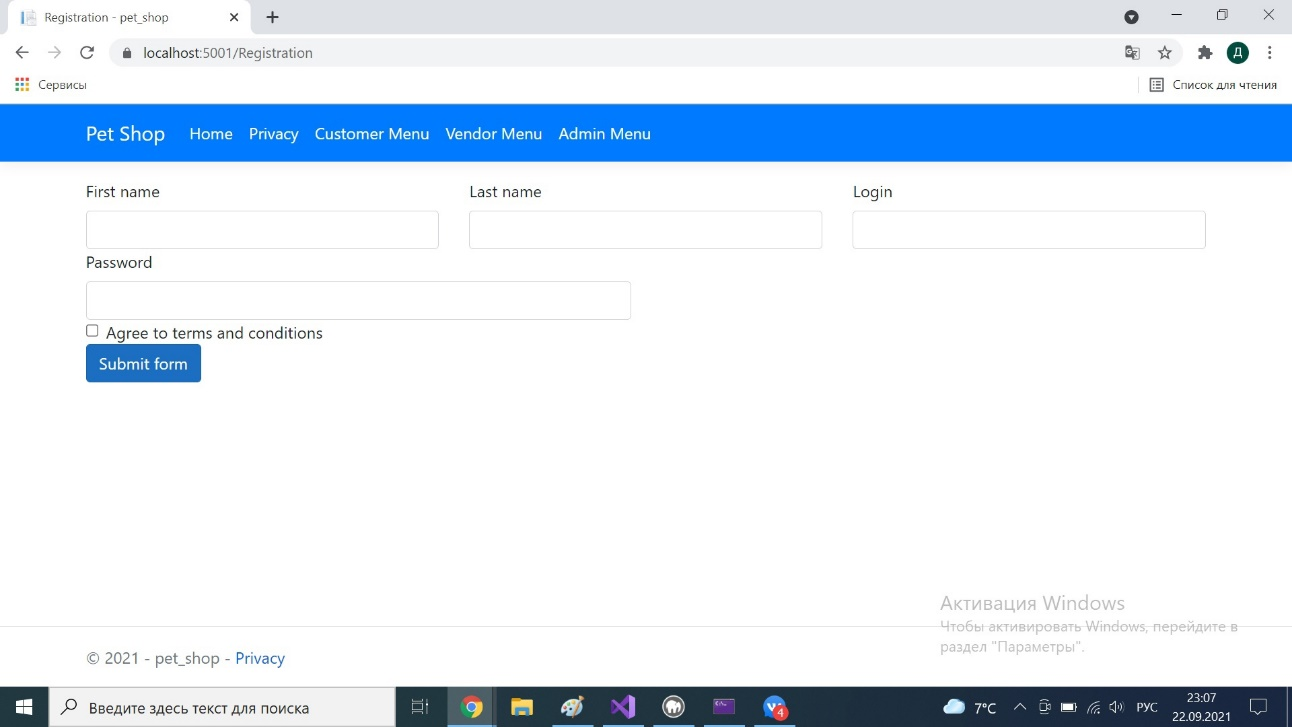
\includegraphics[scale=1]{img/interface1.png}
  \caption{Окно регистрации}
  \label{fig:interface1}
\end{figure}

\begin{figure}[ht!]
  \centering
  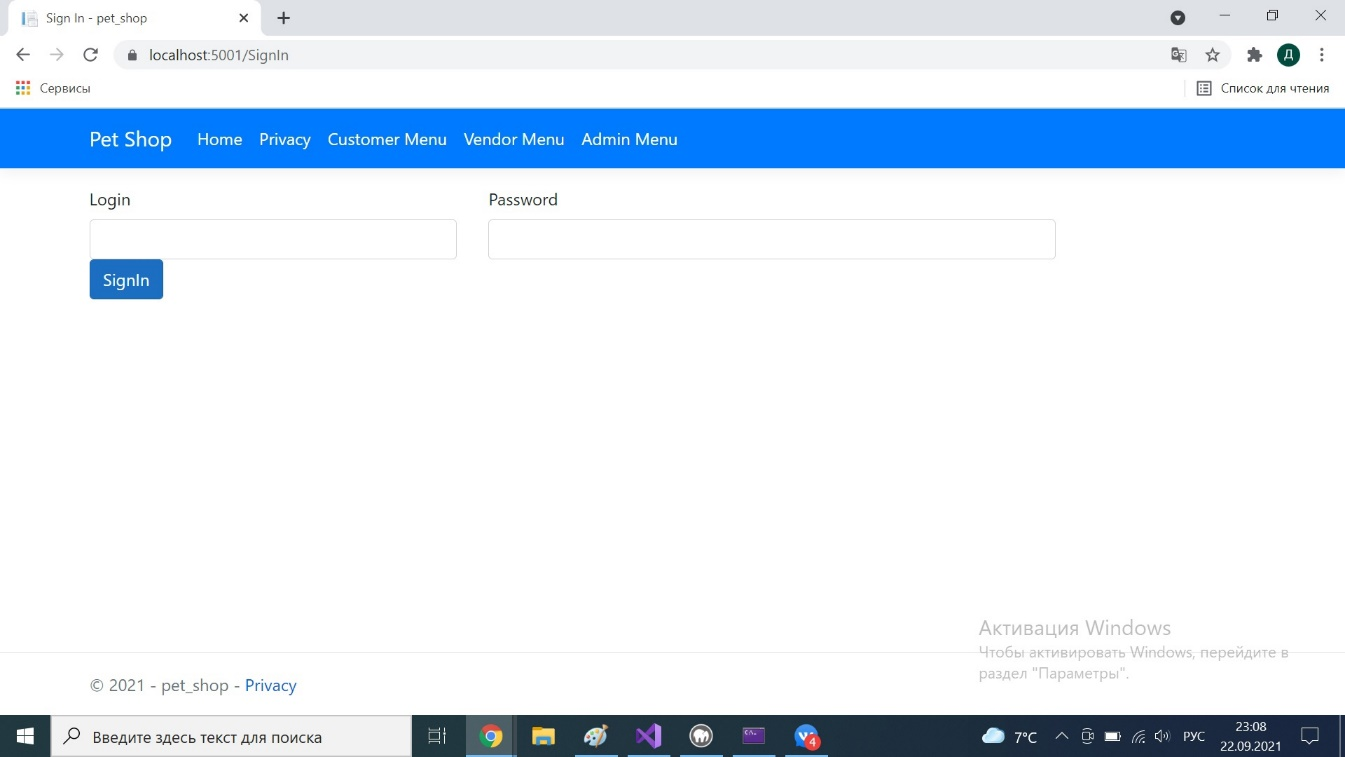
\includegraphics[scale=1]{img/interface2.png}
  \caption{Окно авторизации}
  \label{fig:interface2}
\end{figure}

\newpage

\begin{figure}[ht!]
  \centering
  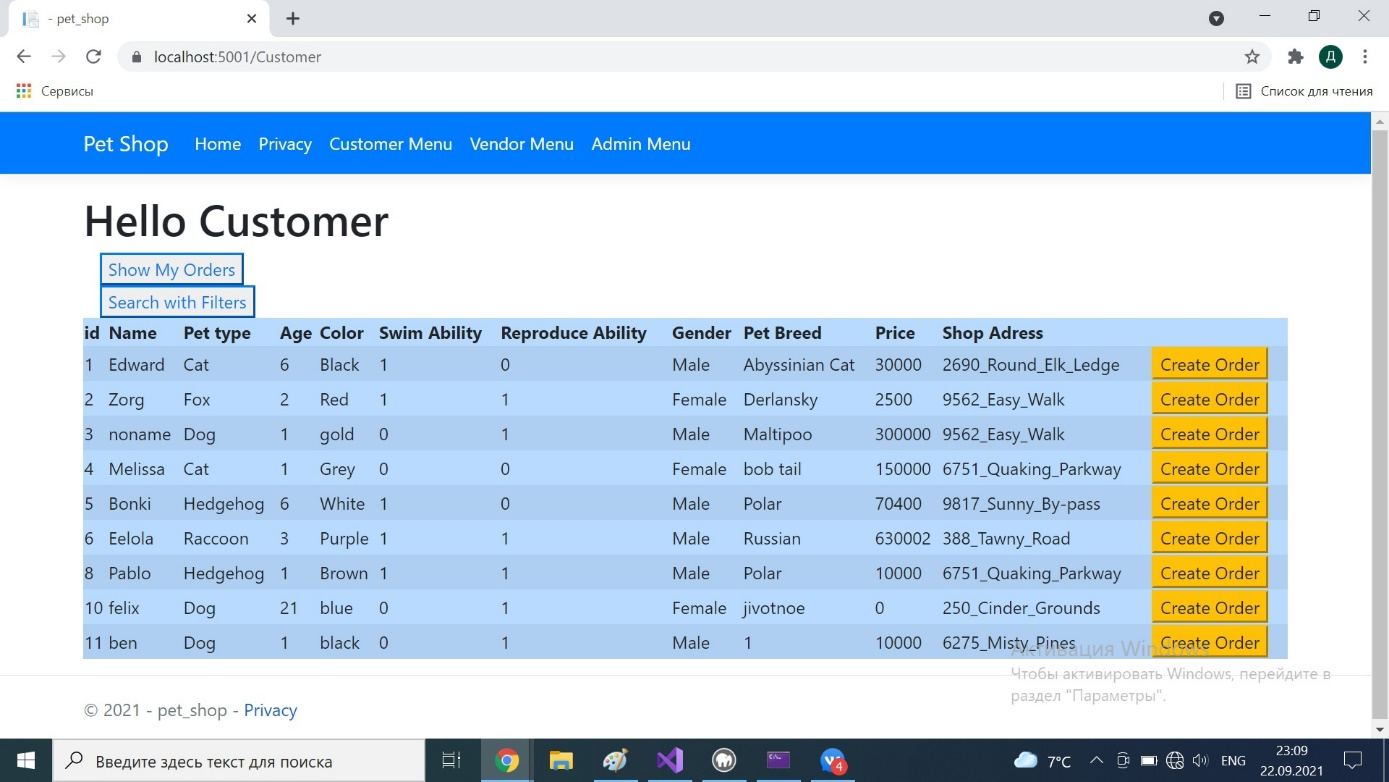
\includegraphics[scale=0.9]{img/interface3.png}
  \caption{Окно покупателя}
  \label{fig:interface3}
\end{figure}

В меню покупателя на рисунке \ref{fig:interface3} можно создавать заказы, а также просматривать доступные товары.

\begin{figure}[ht!]
  \centering
  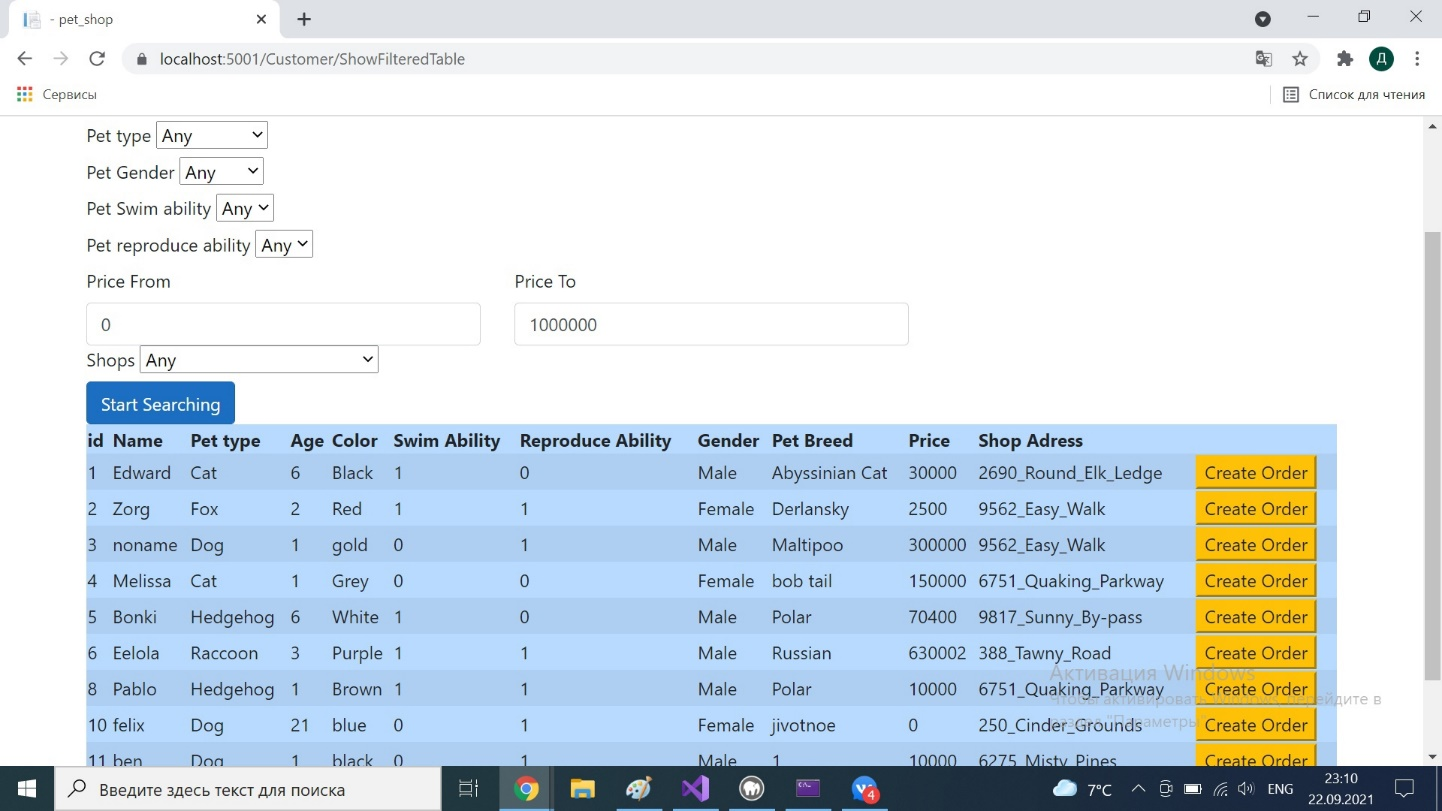
\includegraphics[scale=0.9]{img/interface4.png}
  \caption{Окно поиска товаров с фильтром}
  \label{fig:interface4}
\end{figure}

В окне, изображенном на рисунке \ref{fig:interface4}, можно просматривать товары и делать заказы, только с возможностью выбрать конкретные интересующие покупателя товары.

\newpage

\begin{figure}[ht!]
  \centering
  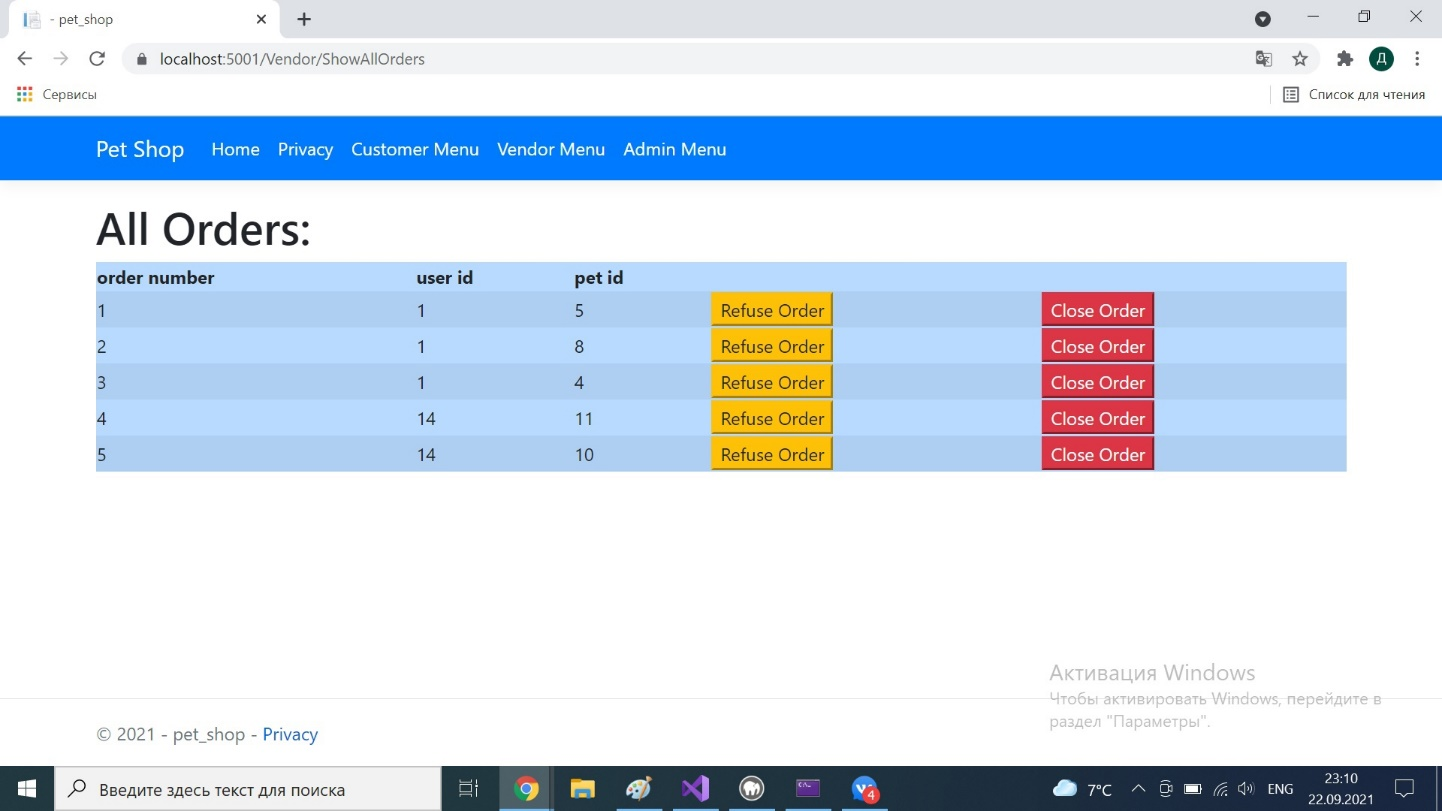
\includegraphics[scale=0.9]{img/interface5.png}
  \caption{Окно продавца}
  \label{fig:interface5}
\end{figure}

В окне продавца на рисунке \ref{fig:interface5} присутствуют все заказы. Есть возможность отклонить заказ, если покупатель не может сделать этого сам или закрытие заказа, что означает, что покупка питомца была совершена.

\begin{figure}[ht!]
  \centering
  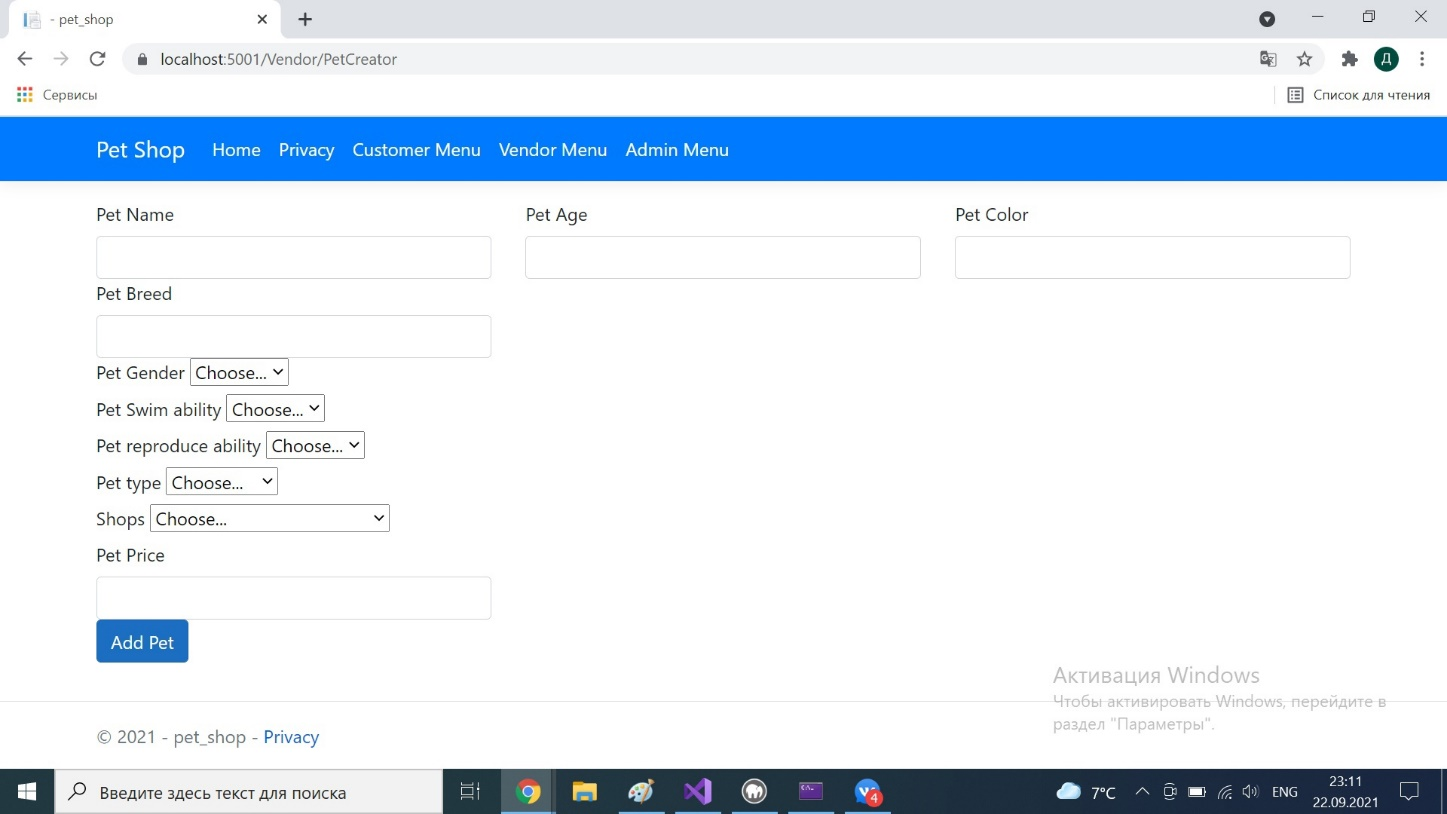
\includegraphics[scale=0.9]{img/interface6.png}
  \caption{Окно создания товара}
  \label{fig:interface6}
\end{figure}

В окне создания товара на рисунке \ref{fig:interface6} продавец может добавить новое животное в список доступных.

\begin{figure}[ht!]
  \centering
  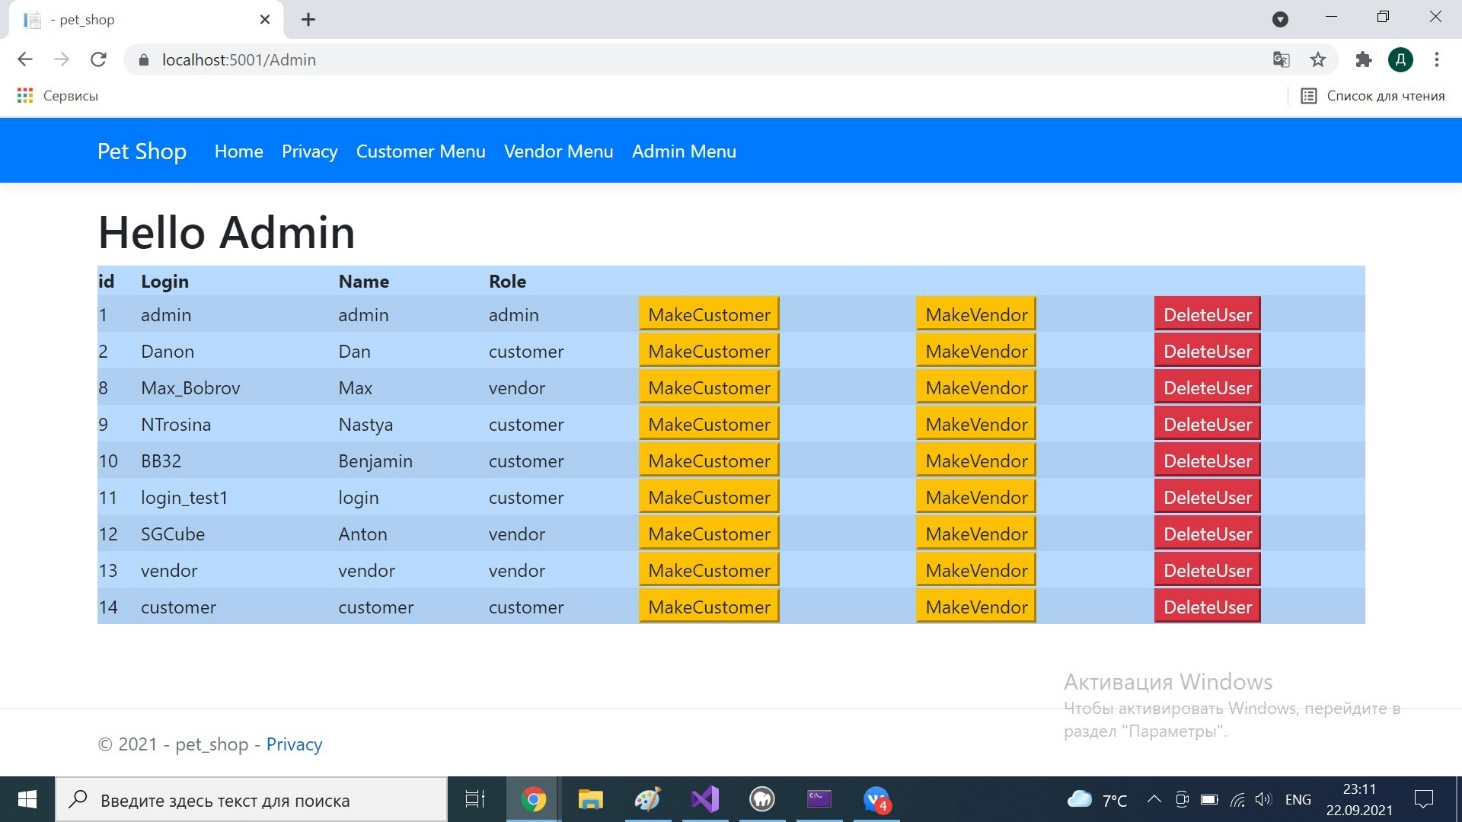
\includegraphics[scale=0.9]{img/interface7.png}
  \caption{Окно администратора}
  \label{fig:interface7}
\end{figure}

Администратор имеет возможность удалять пользователей, либо изменять их роли. В системе администратор зарегистрирован может быть только один.

\newpage

\section{Вывод}
В данном разделе были описаны выбранные средства, среда разработки, язык, СУБД, а также продемонстрирован интерфейс веб-приложения.

    \chapter*{Заключение}
\addcontentsline{toc}{chapter}{Заключение}
В рамках курсового проекта были проанализированы существующие интернет-магазины и их функционал, различные типы баз данных, СУБД, построены диаграммы ER, Use-case для понимания стурктуры и логики будущего ПО.  Далее были подобраны инструменты для разработки, язык программирования, среда, дополнительные утилиты для работы с БД. Для веб-приложения были разработаны функции для работы с БД, Front-end состоящий из нескольких меню, для покупателей, продавцов и администраторов с проверкой прав доступа к ним. Так же меню для создания акаунта и авторизации. После разработано веб-приложение, учитывая проведенную работу.

\hspace{0cm} В данном веб-приложении есть возможности для расширения регистрации со вводом и проверкой электронной почты, функцией восстановления пароля, при его утрате. Для быстрой обратной связи покупателей и продавцов добавить чат, при необходимости консультации.


\begin{thebibliography}{3}
  \addcontentsline{toc}{chapter}{Список литературы}
  \bibitem{web:SQLite}
  Sqlite vs PostgeSql vs MySql. [Электронный ресурс]. - Режим доступа:  https://devacademy.ru/article/sqlite-vs-mysql-vs-postgresql
  
  \bibitem{web:PostgreSQL}
  PostgreSQL, MariaDB и SQLite - сравнение баз данных. [Электронный ресурс]. - Режим доступа:  https://overcoder.net/manuals/postgresql-mariadb-i-sqlite-sravnenie-baz-dannyh
  
  \bibitem{web:MariaDB}
  PostgreSQL, MariaDB и SQLite - сравнение баз данных. [Электронный ресурс]. - Режим доступа: 
  https://skillbox.ru/media/code/entity\_framework/
  
  \bibitem{web:DBTypes}
  Типы БД. [Электронный ресурс]. - Режим доступа:  https://proglib.io/p/11-tipov-sovremennyh-baz-dannyh-kratkie-opisaniya-shemy-i-primery-bd-2020-01-07
  
  \bibitem{web:DBTypes2}
  Типы БД. [Электронный ресурс]. - Режим доступа: https://www.oracle.com/ru/database/what-is-database/
  
  \bibitem{web:IerarchiDB}
  Иерархическая БД, плюсы и минусы. [Электронный ресурс]. - Режим доступа:  https://studbooks.net/2263476/informatika/sostoyat\_preimuschestva\_nedostatki\_ierarhicheskoy\_modeli\_dannyh
  
  \bibitem{web:NetworkDB}
  Сетевая БД, преимущества и недостатки. [Электронный ресурс]. - Режим доступа:  https://life-prog.ru/2\_37690\_setevaya-model-dostoinstva-i-nedostatki.html
  
  \bibitem{web:GraphDB}
  Графовые БД, недостатки. [Электронный ресурс]. - Режим доступа: https://qastack.ru/programming/13046442/comparison-of-relational-databases-and-graph-databases
\end{thebibliography}
\end{document}
